\documentclass[varwidth,border=2pt]{standalone}

% Tikz packages
\usepackage{tikz}
\usetikzlibrary{%
    patterns, plotmarks, backgrounds, shapes, arrows, calc, trees,
    positioning, chains, shapes.geometric, decorations.pathreplacing,
    calligraphy, decorations.pathmorphing, shapes.arrows, bending,
    decorations.markings, quotes, arrows.meta, spy, fit, matrix,
    decorations.text
}

% General includegraphics and colour support
\usepackage{graphicx}
\usepackage{xcolor}

\newdimen\nodeSize
\nodeSize=4mm
\newdimen\nodeDist
\nodeDist=6mm

\makeatletter
\tikzset{
    position/.style args={#1 degrees from #2}{
        at=(#2.#1), anchor=#1+180, shift=(#1:\tikz@node@distance)
    }
}
\makeatother

\tikzset{
dot/.style = {%
    circle, minimum size=#1,
    inner sep=0pt, outer sep=0pt},
    dot/.default = 6pt % size of the circle diameter
}

\definecolor{jpurple}{HTML}{9558B2}
\definecolor{jgreen}{HTML}{389826}
\definecolor{jred}{HTML}{CB3C33}

\begin{document}
    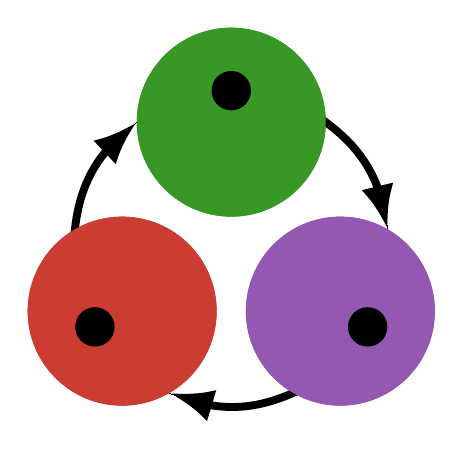
\begin{tikzpicture}[%
        every edge/.style = {draw, -Latex, line width=1.0mm}
    ]
        % Initialize starting node
        \node[] (start) { };

        % Define the Julia dot coordinates
        \path (start) ++(+90:16mm)   node[] (up)     { };
        \path (start) ++(-30:16mm)   node[] (right)  { };
        \path (start) ++(-150:16mm)  node[] (left)   { };

        % Define the inner "particle" dot coordinates
        \path (start) ++(+90:20mm)   node[] (up2)     { };
        \path (start) ++(-30:20mm)   node[] (right2)  { };
        \path (start) ++(-150:20mm)  node[] (left2)   { };

        % Julia dots
        \node[dot=24mm,fill=jgreen]  at (up.center)    (C1) {};
        \node[dot=24mm,fill=jpurple] at (right.center) (C2) {};
        \node[dot=24mm,fill=jred]    at (left.center)  (C3) {};

        % Black circle around Julia dots with cycling arrows
        \node[dot=40.0mm,fill=none,draw,line width=0.0mm] at (start.center)  (C4) {};
        \draw (C4.176) edge[bend left=24] (C4.127);
        \draw (C4.56) edge[bend left=24] (C4.7);
        \draw (C4.296) edge[bend left=24] (C4.247);

        % Diagnostic lines (for modifying logo)
        %\draw (C4.center) -- (C4.176);
        %\draw (C4.center) -- (C4.124);
        %\draw (C4.center) -- (C4.150);

        %\draw (C4.center) -- (C4.56);
        %\draw (C4.center) -- (C4.4);
        %\draw (C4.center) -- (C4.30);

        %\draw (C4.center) -- (C4.296);
        %\draw (C4.center) -- (C4.244);
        %\draw (C4.center) -- (C4.270);

        % Julia dots (to cover cycling arrows)
        \node[dot=24mm,fill=jgreen]  at (up.center)    (C1) {};
        \node[dot=24mm,fill=jpurple] at (right.center) (C2) {};
        \node[dot=24mm,fill=jred]    at (left.center)  (C3) {};

        % Inner "particle" dots
        \node[dot=5mm,fill=black]    at (up2.center)    () {};
        \node[dot=5mm,fill=black]    at (right2.center) () {};
        \node[dot=5mm,fill=black]    at (left2.center)  () {};

    \end{tikzpicture}
\end{document}

